\section{Теоретические предпосылки}

\begin{frame}{Применение радиометок в SCADA-системе}
    \centering
    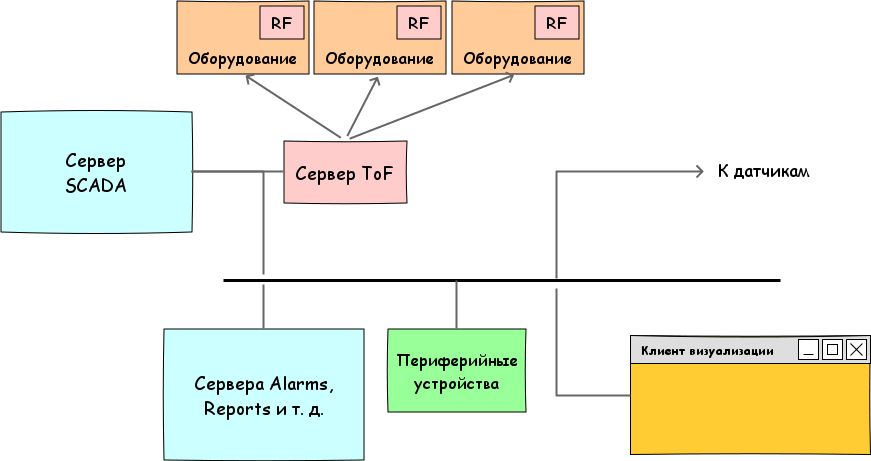
\includegraphics[width=1\linewidth]{../Figures/scada.png}
\end{frame}

\begin{frame}{Диапазон радиоволн}
    \centering
    \begin{longtable}[c]{|c|c|c|}
        \hline
        \textbf{Диапазон} & \textbf{Частота} & \textbf{Длина волны}\\
        \hline
        \endfirsthead
        \hline
        \textbf{Диапазон} & \textbf{Частота} & \textbf{Длина волны}\\
        \hline
        \endhead
            Сверхдлинные <<СДВ>> & 3 -- 30 кГц & 100 -- 10 км\\
            \hline
            Длинные <<ДВ>> & 30 -- 300 кГц & 10 -- 1 км\\
            \hline
            Средние <<СВ>> & 300 -- 3000 кГц & 1000 -- 100 м\\
            \hline
            Короткие <<КВ>> & 3 -- 30 МГц & 100 -- 10 м\\
            \hline
            Ультракороткие <<УКВ>> & 30 МГц -- 6000 ГГц & 10 м -- 0.05 мм\\
            \hline
    \end{longtable}

    Ультракороткие радиоволны

    \begin{longtable}[c]{|c|c|c|}
        \hline
        \textbf{Диапазон} & \textbf{Частота} & \textbf{Длина волны}\\
        \hline
        \endfirsthead
        \hline
        \textbf{Диапазон} & \textbf{Частота} & \textbf{Длина волны}\\
        \hline
        \endhead
            Метровые <<МВ>> & 30 -- 300 МГц & 10 -- 1 м\\
            \hline
            Дециметровые <<ДМВ>> & 300 -- 3000 МГц & 10 -- 1 дм\\
            \hline
            Сантиметровые <<СМВ>> & 3 -- 30 ГГц & 10 -- 1 см\\
            \hline
            Миллиметровые <<ММВ>> & 30 -- 300 ГГц & 10 -- 1 мм\\
            \hline
            Субмиллиметровые <<СММВ>> & 300 -- 6000 ГГц & 1 -- 0.05 мм\\
            \hline
    \end{longtable}
\end{frame}

\begin{frame}{Модуляция}
    \begin{columns}
        \column{.4\textwidth}
        \centering
        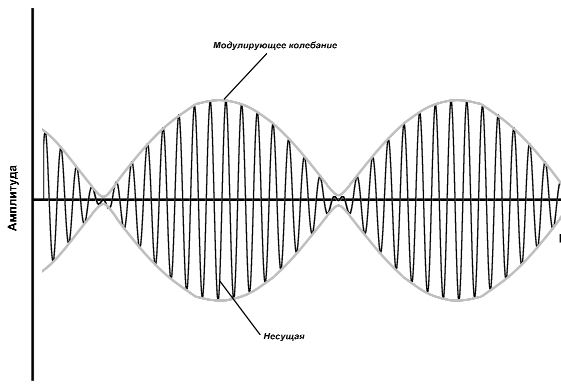
\includegraphics[width=1\linewidth]{../Figures/am.jpg}

        Амплитудная модуляция
        \column{.6\textwidth}
        \centering
        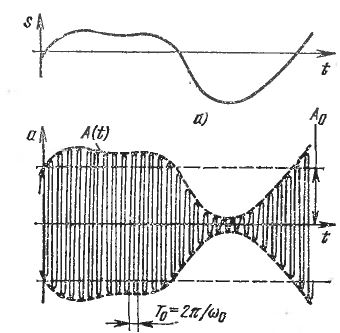
\includegraphics[width=.7\linewidth]{../Figures/amclose.jpg}

        АМ-сигнал
    \end{columns}
\end{frame}

\begin{frame}{Устройство радиопередатчика}
    \begin{columns}
        \column{.4\textwidth}
        \centering
        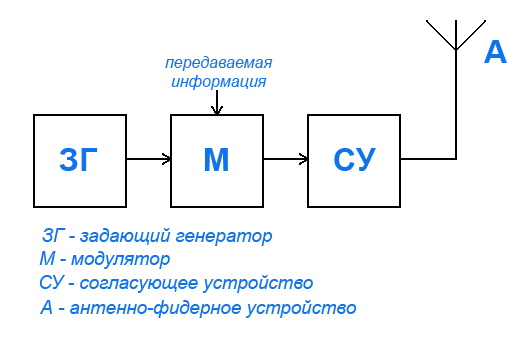
\includegraphics[width=1\linewidth]{../Figures/radiostruct.jpg}

        Структурная схема радиопередатчика
        \column{.6\textwidth}
        \centering
        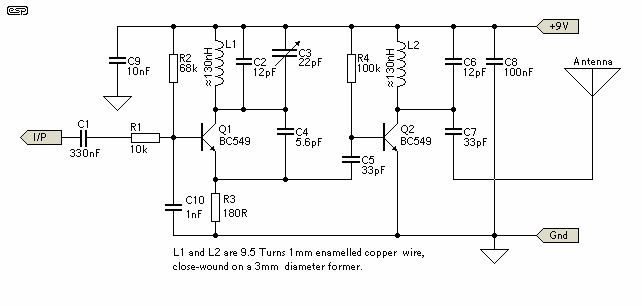
\includegraphics[width=1\linewidth]{../Figures/rfcircuit.png}

        Принципиальная схема радиопередатчика
    \end{columns}
\end{frame}

\section{Реализация метода Time of Flight}

\begin{frame}{Функциональная схема \textit{Time of Flight} устройства}
    \begin{columns}
        \column{.6\textwidth}
        \centering
        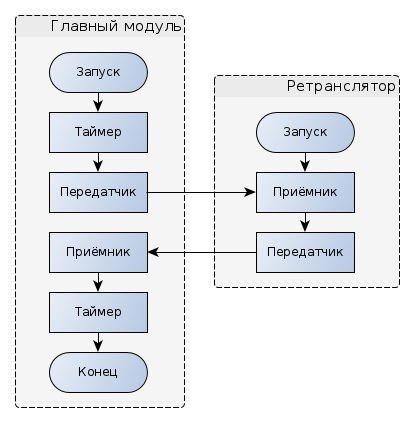
\includegraphics[width=1\linewidth]{../Figures/tofscheme.png}

        \column{.4\textwidth}
        \centering
        \large{$t = \frac{T_f}{2}$}

        \large{$f = \frac{1}{T_f} = \frac{c}{S}$}
    \end{columns}
\end{frame}

\begin{frame}{Функциональная схема метода <<накопления>> ToF}
    \centering
    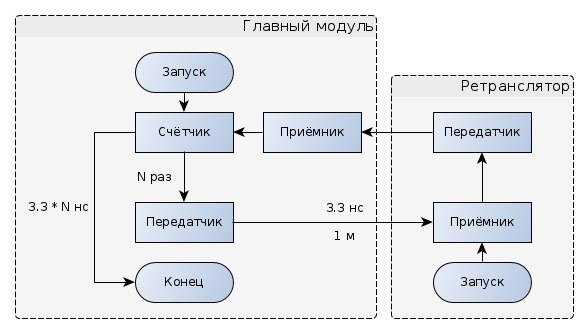
\includegraphics[width=.8\linewidth]{../Figures/accscheme.png}

    \vfill

    $T_f = \frac{1}{300.000.000} = 3.3$ нс.

    $t_w = \frac{\Delta\tau}{T_f} = \frac{50 \cdot 10^{-6}~\textrm{с}}{3.3 \cdot 10^{-9}~\textrm{с}} = 15151~\textrm{с} = 252~\textrm{мин} = 4.2~\textrm{ч}$
\end{frame}

\begin{frame}{Проблемы реализации ToF-устройства}
    \begin{columns}
        \column{.8\textwidth}
        \centering
        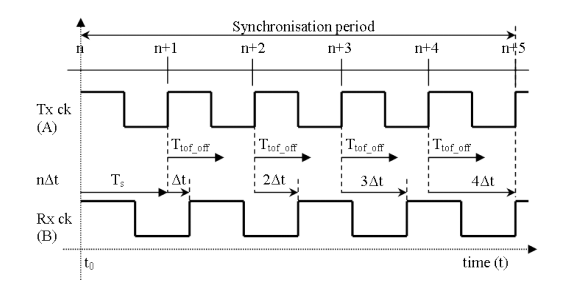
\includegraphics[width=1.1\linewidth]{../Figures/sync.png}

        \column{.2\textwidth}
        \centering
        $\sigma_r^2 >= \frac{c^2}{\frac{4 \pi^2 B^2 E_S}{N_0}}$
    \end{columns}
\end{frame}

\begin{frame}{Нижняя граница диапазона ToF-ошибки}
    \centering
    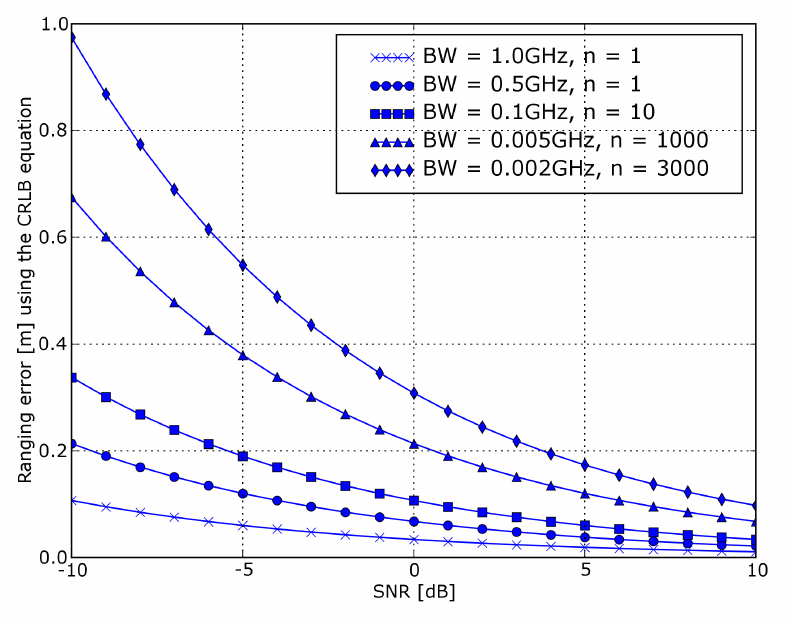
\includegraphics[width=.8\linewidth]{../Figures/cramer.png}
\end{frame}

\section{Подбор оборудования}

\begin{frame}{Структурная схема микроконтроллера}
    \begin{columns}
        \column{.6\textwidth}
        \centering
        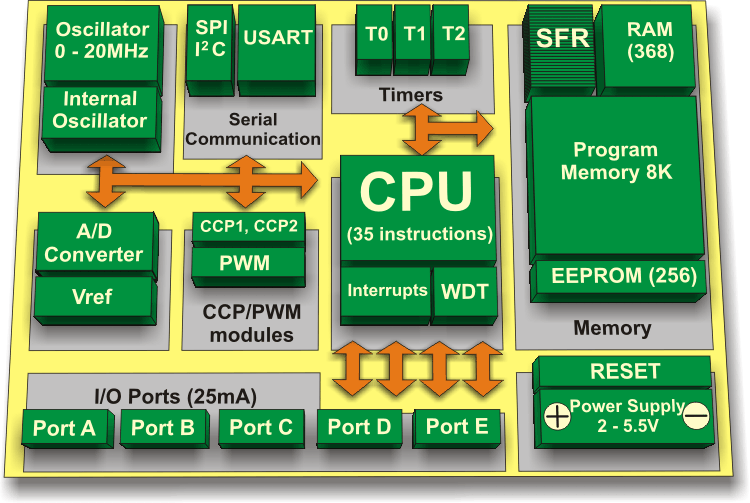
\includegraphics[width=1.1\linewidth]{../Figures/microstruct.png}

        \column{.4\textwidth}
        \centering
        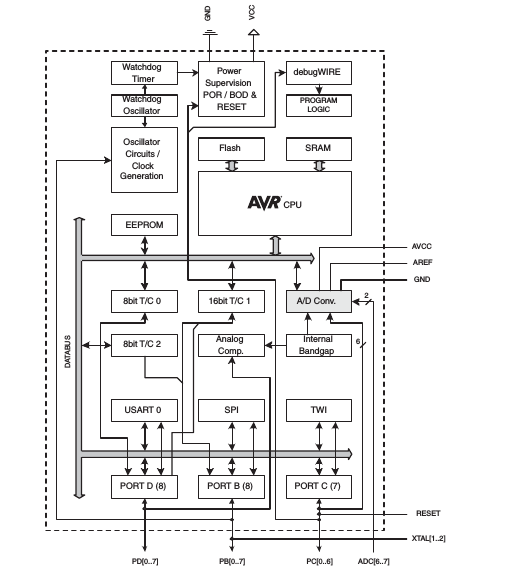
\includegraphics[width=1.1\linewidth]{../Figures/atmegablock.png}
    \end{columns}

    \centering
\end{frame}

\begin{frame}{Технические характеристики Arduino UNO и Arduino MEGA}
    \centering
    \begin{longtable}[c]{|p{2in}|c|c|}
        \hline
        \textbf{Параметр} & \textbf{UNO} & \textbf{MEGA}\\
        \hline
        \endfirsthead
        \hline
        \textbf{Параметр} & \textbf{UNO} & \textbf{MEGA}\\
        \hline
        \endhead
            Микроконтроллер & ATmega328 & ATmega2560\\
            \hline
            Оперируемое напряжение & \multicolumn{2}{c|}{5 В}\\
            \hline
            Входное напряжение (реккомендуемое) & \multicolumn{2}{c|}{7 -- 12 В}\\
            \hline
            Входное напряжение (максимальное) & \multicolumn{2}{c|}{6 -- 20 В}\\
            \hline
            Цифровые входы/выходы & 14 (~6) & 54 (~14)\\
            \hline
            Аналоговые входы & 6 & 16\\
            \hline
            Постоянные ток на 1 вход/выход & \multicolumn{2}{c|}{40 мА}\\
            \hline
            Постоянный ток на вход 3.3 В & \multicolumn{2}{c|}{50 мА}\\
            \hline
            Память & 32 Кб & 256 Кб\\
            \hline
            Частота задающего генератора & \multicolumn{2}{c|}{16 МГц}\\
            \hline
    \end{longtable}
\end{frame}

\begin{frame}{Спецификация Arduino UNO}
    \centering
    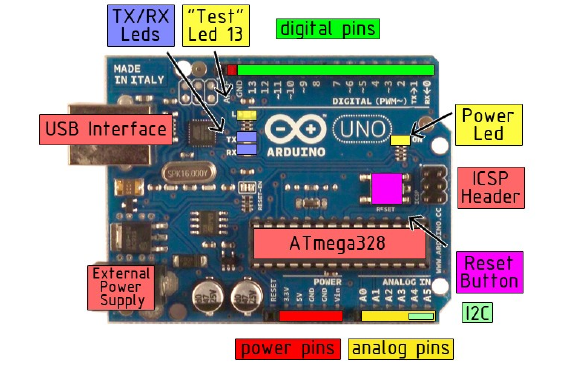
\includegraphics[width=.8\linewidth]{../Figures/specuno.png}
\end{frame}

\begin{frame}{Блок-схема Time of Flight устройства}
    \centering
    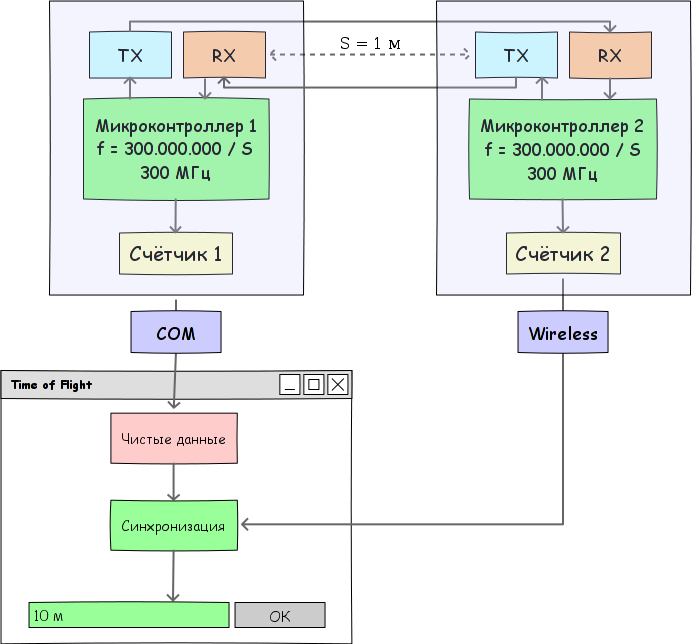
\includegraphics[width=.6\linewidth]{../Figures/commonscheme.png}
\end{frame}

\begin{frame}{Подключение модуля ToF}
    \begin{columns}
        \column{.5\textwidth}
        \centering
        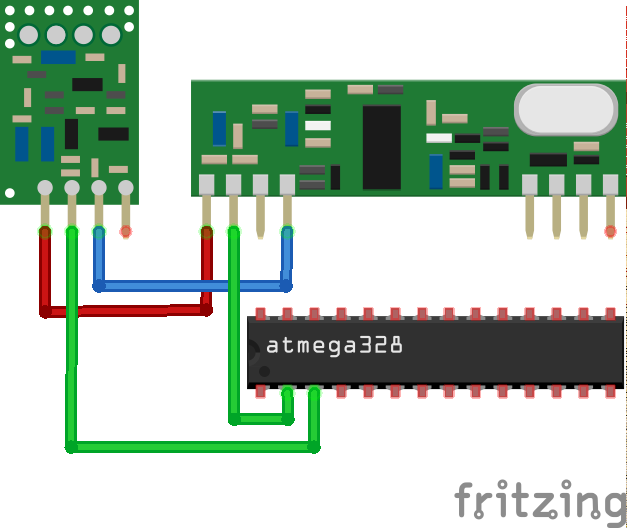
\includegraphics[width=1\linewidth]{../Figures/hardscheme.png}

        Общий вид подключения
        \column{.5\textwidth}
        \centering
        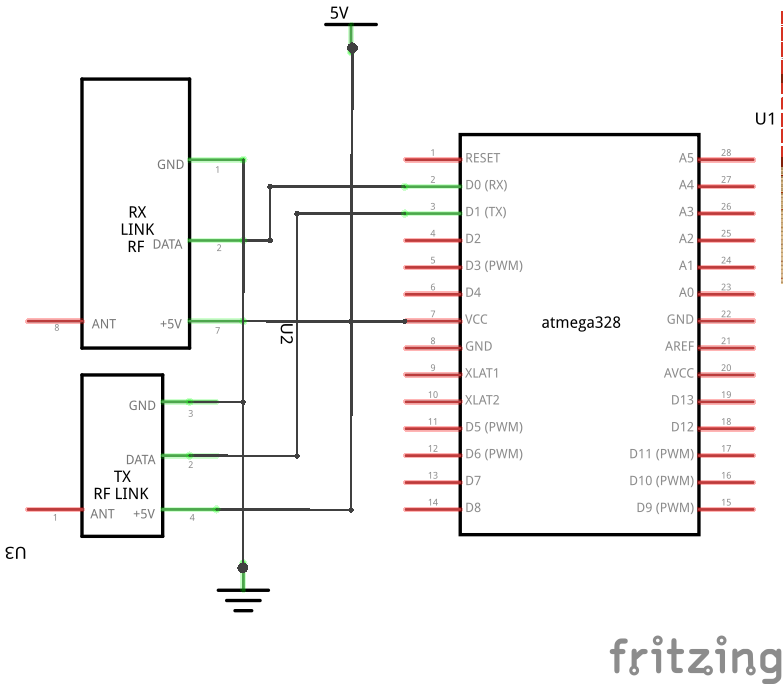
\includegraphics[width=1\linewidth]{../Figures/circscheme.png}

        Схемотехника подключения
    \end{columns}
\end{frame}

\begin{frame}{Алгоритм работы устройства}
    \centering
    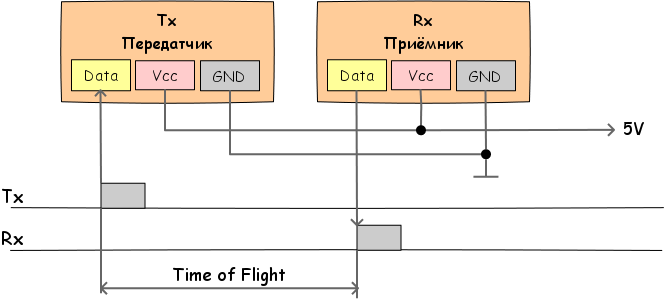
\includegraphics[width=1\linewidth]{../Figures/physalg.png}
\end{frame}

\section{Разработка программной модели}

\begin{frame}{Функциональная схема программных модулей}
    \centering
    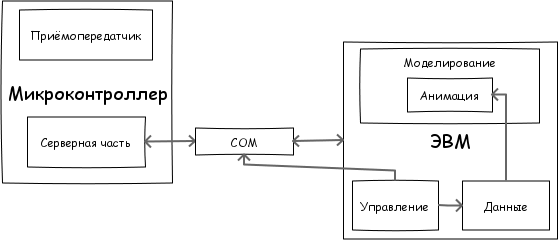
\includegraphics[width=1\linewidth]{../Figures/softwarefunc.png}
\end{frame}

\begin{frame}{Алгоритм программной модели модуля ToF}
    \begin{columns}
        \column{.5\textwidth}
        \centering
        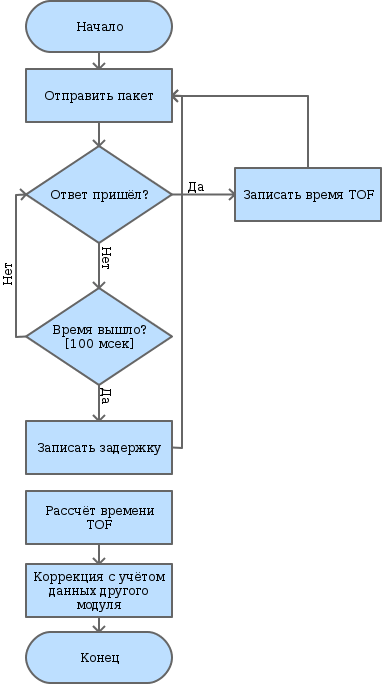
\includegraphics[width=.6\linewidth]{../Figures/codeblock.png}

        Модуль-сервер
        \column{.5\textwidth}
        \centering
        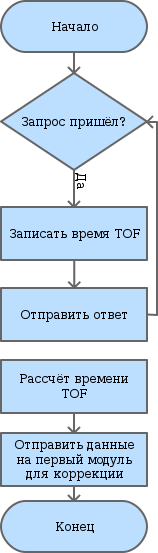
\includegraphics[width=.3\linewidth]{../Figures/codeblock2.png}

        Модуль-клиент
    \end{columns}
\end{frame}

\section{Анализ помех оборудования и программной среды}

\begin{frame}{Частотный анализ Arduino}
    \begin{columns}
        \column{.5\textwidth}
        \centering
        Работа с Arduino
        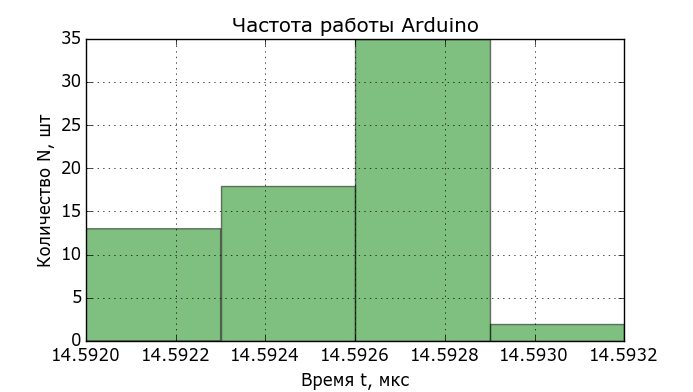
\includegraphics[width=1\linewidth]{../Figures/ardhist.png}
        \vfill
        $f = \frac{n}{t} = \frac{10000}{145928 \cdot 10^{-6}} = 68.5~\textrm{кГц}$

        \column{.5\textwidth}
        \centering
        Работа с портами ATMega
        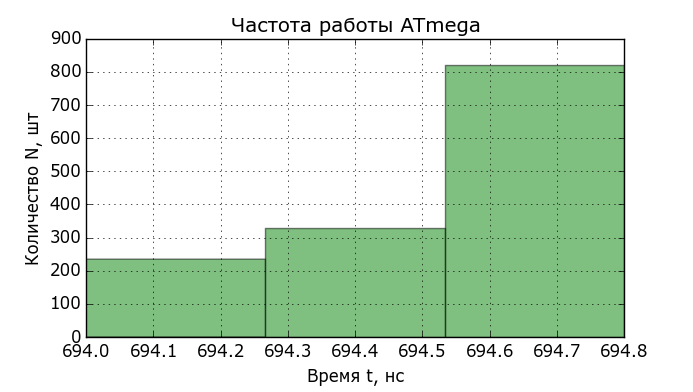
\includegraphics[width=1\linewidth]{../Figures/athist.png}
        \vfill
        $f = \frac{n}{t} = \frac{10000}{6948 \cdot 10^{-6}} = 1.44~\textrm{МГц}$
    \end{columns}

\end{frame}

\begin{frame}{Диаграмма портов ATMega328 в Arduino}
    \centering
    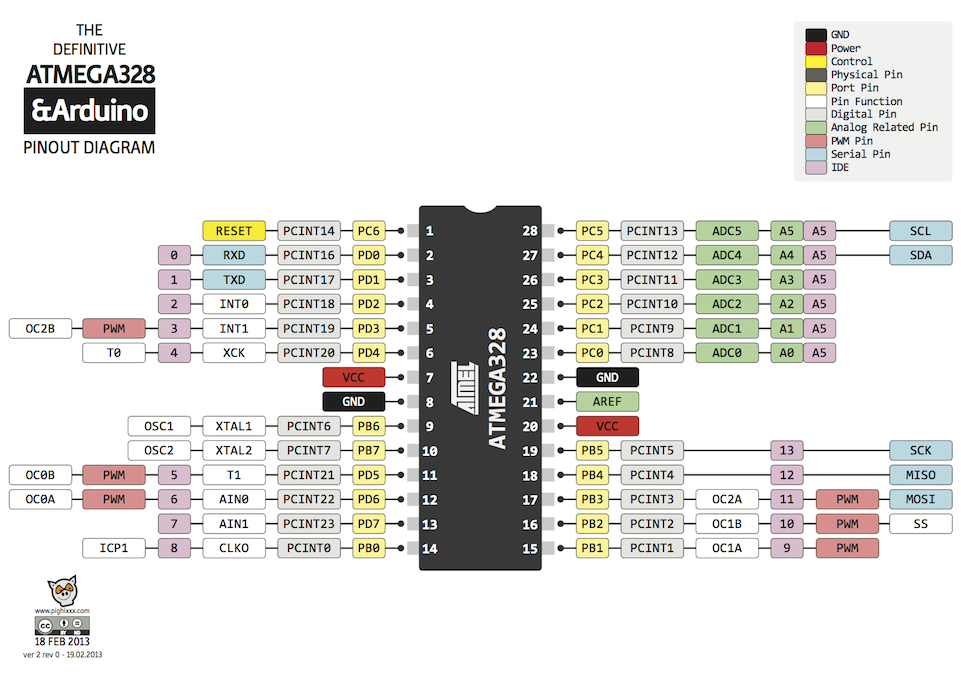
\includegraphics[width=1\linewidth]{../Figures/a328diagram.png}
\end{frame}

\section{Технико-экономические показатели проекта}

\begin{frame}{Технико-экономические показатели проекта}
    \centering
    \begin{figure}[ht]
        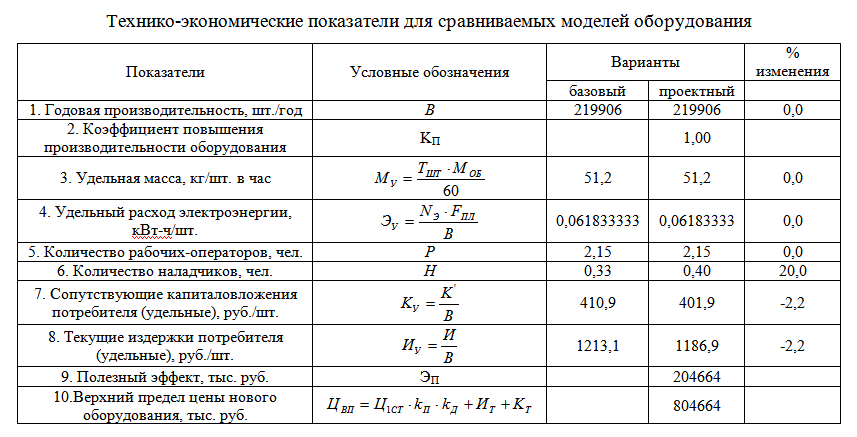
\includegraphics[width=1\linewidth]{Figures/econtable.png}
    \end{figure}
\end{frame}
